%!TEX root = vorlage.tex

\section{Models}

In this practical, we were examining deep neural network models for semantic
segmentation. The most basic neural network model is a so called
\textit{multilayer Perceptron} (\textit{MLP}). MLPs consist of an input layer,
multiple hidden layers and an output layer. Each layer consists of nodes. The
number of nodes of the input layer is determined by the features and the number
of output nodes is determined by the classes. The number of nodes in the hidden
layers can be arbitrary large, but is typically between 0.25 and 3 times the
number of the layer before. The parameters which get adjusted during the
training of a model are called \textit{weights}. One weight is between two
neurons of neighboring layers.

Each node has an activation function. Two functions which are used very often
are the \textit{sigmoid function} and the \textit{rectified linear function}.

The sigmoid activation function is

\[\varphi: \mathbb{R} \rightarrow (0, 1) \qquad \varphi(x) = \frac{1}{1 + e^{-x}}\]

while rectified linear units (commonly abbreviated with ReLU) have the
activation function

\[\varphi: \mathbb{R} \rightarrow [0, \infty) \qquad \varphi(x) = \max(0, x)\]

A more detailed introduction to MLPs can be found in~\cite{Mitchell1997}.

\subsection{Convolutional Neural Networks}
One of the most important extensions of MLPs are so called
\textit{Convolutional Neural Networks} (CNNs). Those introduce two new layer types
besides the fully connected layers: convolutional layers and pooling layers.
Each convolutional layer has $k \in \mathbb{N}_{\geq 1}$ filters of size $p
\times p \times c$, where $p \in \mathbb{N}_{\geq 1}$ is a design choice and $c
\in \mathbb{N}_{\geq 1}$ is the number of channels of the layer before. The
input layer has typically three channels: Red, green, blue (RGB). When $k$
filters get applied in layer $A$, then the output of layer $A$ has $k$
channels.\\
The parameters which get adjusted during training in convolutional layers are
the weights of the filters. A layer with $k$ filters of size
$p \times p \times c$ has $k \cdot p^2 \cdot c$ weights which get adjusted.

Convolutions produce an output which is smaller than their input, as one can see
in~\cref{fig:convolution-size}.

\begin{figure}[ht]
    \centering
    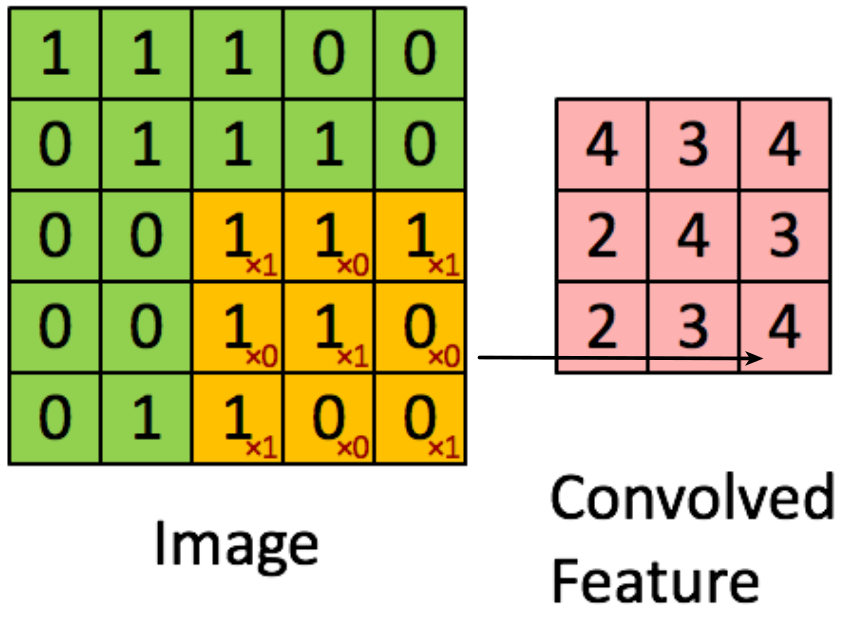
\includegraphics[width=\linewidth]{images/convolution-schematic.png}
    \caption{A $5 \times 5$ image convolved with a $3 \times 3$ filter becomes
             a $3 \times 3$ image as the filter size minus one gets removed
             from the input image size.\\
             Image source:~\cite{Cyfoo}}
    \label{fig:convolution-size}
\end{figure}

Sometimes it is desired to get an output of the same size as the input. In this
case the image is padded with $\frac{\text{filter size} - 1}{2}$ in each
direction. Commonly, the padding is done with zeroes.

The pooling layers do not learn any parameter. They reduce the data being
processed by the network by grouping it. Pooling layers have four hyperparameters:
the pooling function, the pooling size, the strides and the border mode.
The pooling size gives the size of the region to which the pooling function
gets applied. Typically, $3 \times 3$ pooling is chosen. For those four~pixels
the maximum function is chosen. Another option is average pooling. The stride
is the parameter which reduces the amount of processed data. A stride of $(2, 2)$
is used which has the effect of reducing the data to $\nicefrac{1}{4}$th of
the original amount.

There are a couple of well-known image classification networks for which both,
the architecture and the weights are available. One of those networks is called
VGG-16 (for \textit{Visual Geometry Group})~\cite{KarenSimonyan,simonyan2014very}.


\subsection{Fully Convolutional Neural Networks}

Fully Convolutional Networks (FCNs) were introduced by~\cite{long2015fully}.
They were shown to improve performance in semantic segmentation tasks over
standard convolutional neural networks (CNNs).

FCNs combine four ideas:

\begin{enumerate}
    \item Train an image classification network for $k$ classes,
    \item interpret this network as $k$ filters of a single, non-linear
          convolution,
    \item apply those filters to images of arbitrary size to receive a
          coarse heat map for the $k$ classes.
    \item Finally, train an upsampling network to get a fine-grained semantic
          segmentation.
\end{enumerate}

Upsampling is realized by padding and convolution as visualized
in~\cref{fig:upsampling}. It is worth emphasizing that this upsampling is
learned.

\begin{figure}[ht]
    \centering
    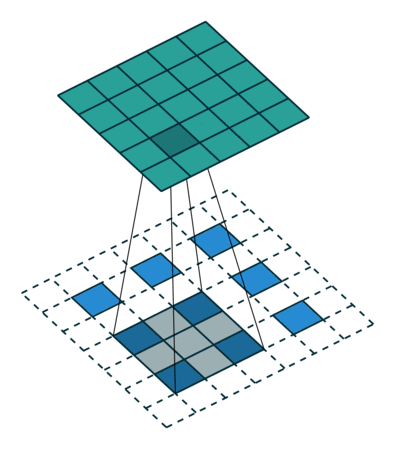
\includegraphics[width=\linewidth]{images/upsampling2-16.png}
    \caption{Upsampling: The blue input gets padded by the white cells. Then
             a convolution is applied --- visualized in gray --- to produce
             the green output.\\
             Image source:~\cite{vdumoulin2016}}
    \label{fig:upsampling}
\end{figure}

